\subsection{Studies in the Highly Restricted Phase Space} % (fold)
\label{sub:small_window_studies}

Removing the discrimination power of $\tau_{21}$ and the jet mass in Sec.~\ref{sub:flat_hypercube_studies} allowed us to quantify the unique discrimination power learned by the neural networks.  However, it does not tell us what information is learned.  Another way to quantify the unique information learned by the network that also provides useful information about physical information learned by the network is to restrict the considered phase space such that $\tau_{21}$ and the jet mass distributions do not vary appreciably over the redacted space.  Figure~\ref{fig:meanImagesWindow} shows the average signal and background jet image in three small windows of $\tau_{21}$, the jet mass, and the jet $p_T$.  In all three windows, the jet mass is restricted to be between 79 GeV and 81 GeV and the jet $p_T$ is required to be in the interval [250,260] GeV.  The three windows are then defined by their value of $\tau_{21}$: [0.19,0.21] in the most two-prong-like case, [0.39,0.41] in a region with likelihood ratio near unity and [0.59,0.61] in a mostly one-prong-like case.  The key physics features of the jets falling in these windows are easily visualized from the average jet images.  The most striking observation is that in these three windows, signal jets look very similar to background jets.  When $\tau_{21}\in[0.19,0.21]$, both signal and background jets have a second subjet that is distinct from the leading subjet and this is washed out as the value of $\tau_{21}$ increases.  

The differences between images in these small windows tells us about what information {\it could be learned} by the networks beyond $\tau_{21}$ and the jet mass.  Since the differences are subtle, the average difference is explicitly computed and plotted in Fig.~\ref{fig:meanImagesWindow2} for the three narrow windows of $\tau_{21}$.  In the window with $\tau_{21}\in[0.19,0.21], there are five features: a localized blue patch in the bottom center, a localized red patch just above that, a red diffuse region between the red patch and the center and then a blue dot just left of center surrounded by a red shell to the right.  Each of these have a physics meaning: the lower two localized patches give information about the orientation of the second subjet $(\Delta R)$ which is slightly wider for the QCD jets which need a slightly wider angle to satisfy the mass requirement.  The red diffuse region just above the localized patches is likely an indication of colorflow: the $W$ bosons are color singlets compared to the color octet gluon jet background, and thus we expect the radiation pattern to be mostly between the two subjets for the $W$.  There is a similar story for all the features in each of the plots in Fig.~\ref{fig:meanImagesWindow2}.

\begin{figure}[bt]
  \begin{center}
  
        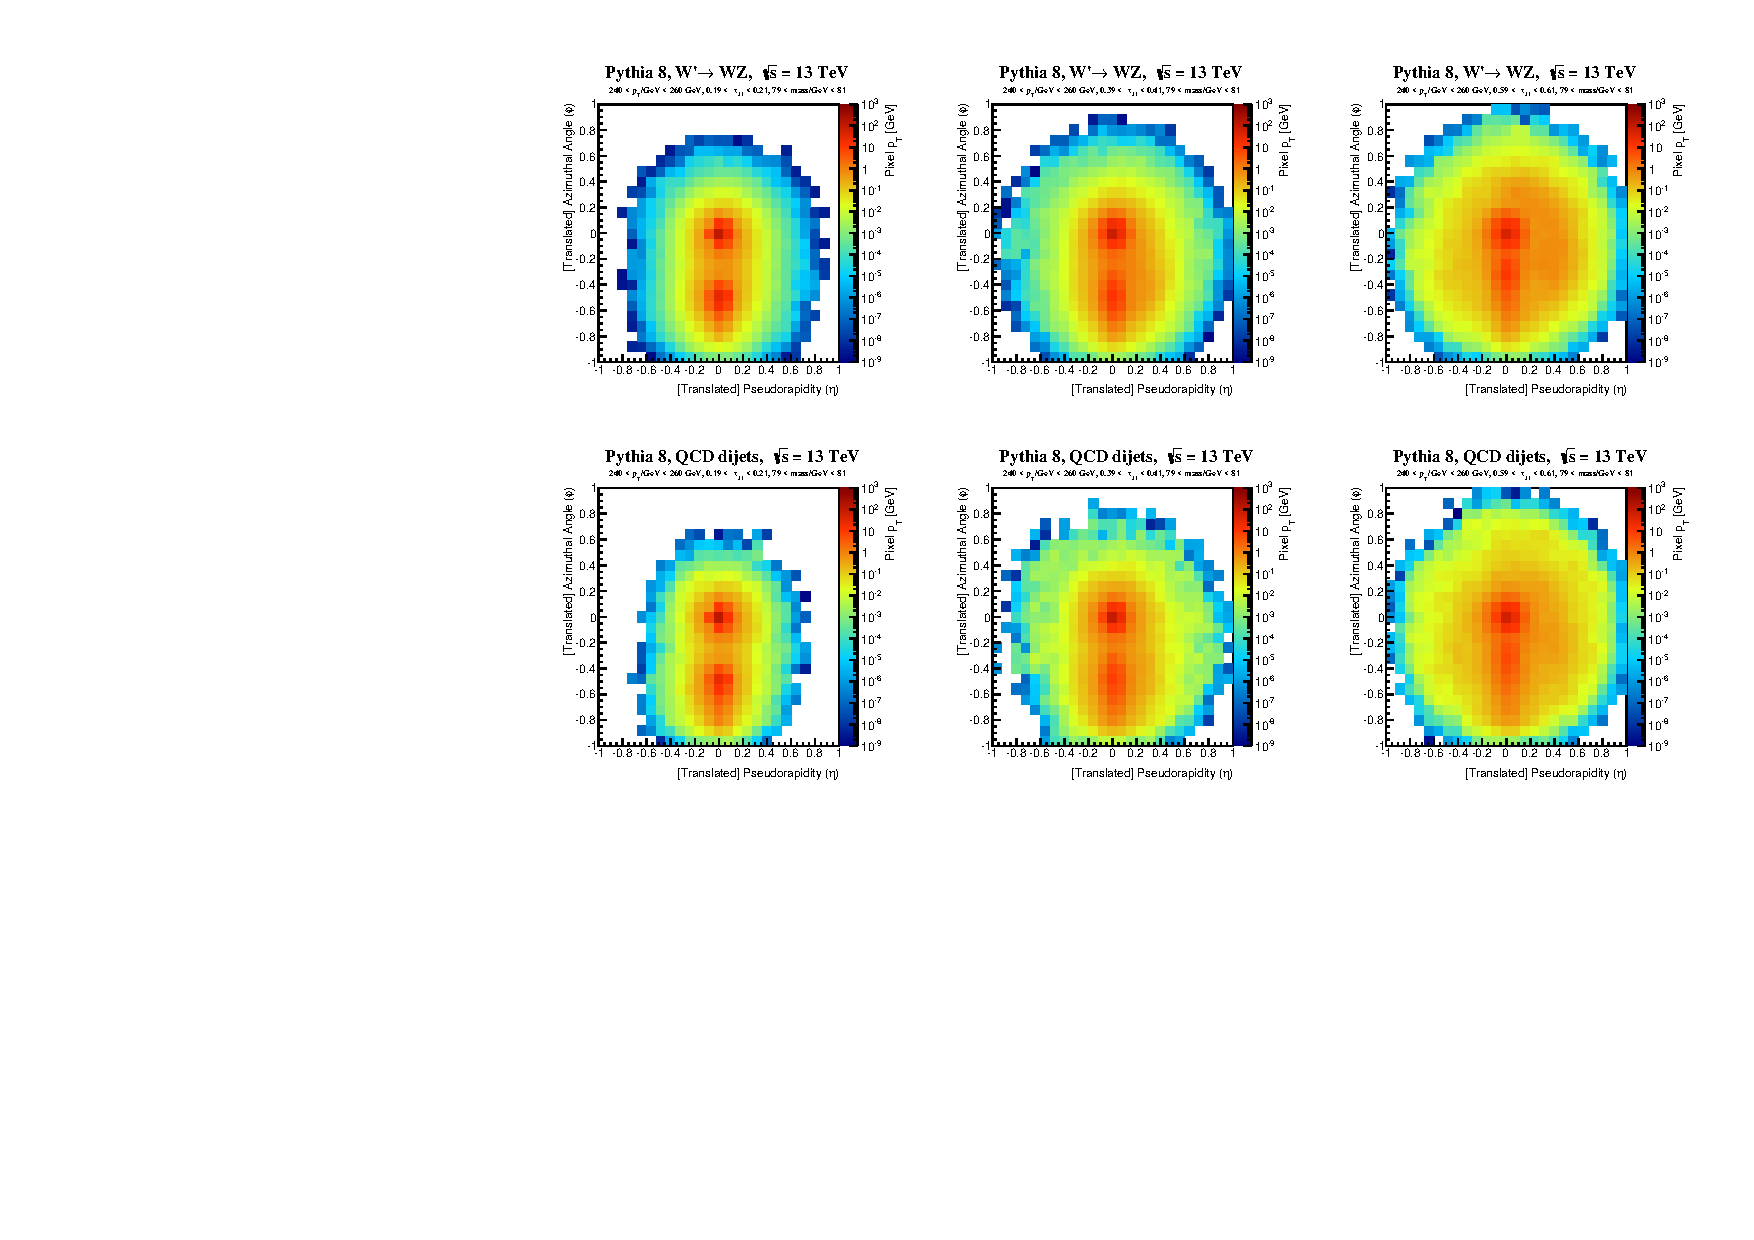
\includegraphics[width=0.99\textwidth]{figures/averages_fixed_nonorm.pdf}

      \caption{
        $W'\rightarrow WZ$ (top) and QCD (bottom) average jet-images in three small windows of $\tau_{21}$: [0.19, 0.21] (left), [0.39, 0.41] (middle), and [0.59, 0.61] (right).  In all cases, jet mass is restricted to be between 79 GeV and 81 GeV and the jet $p_T$ is required to be in the interval [250,260] GeV.
        \label{fig:meanImagesWindow} 
      }
    \end{center}
\end{figure}  

\begin{figure}[bt]
  \begin{center}
  
        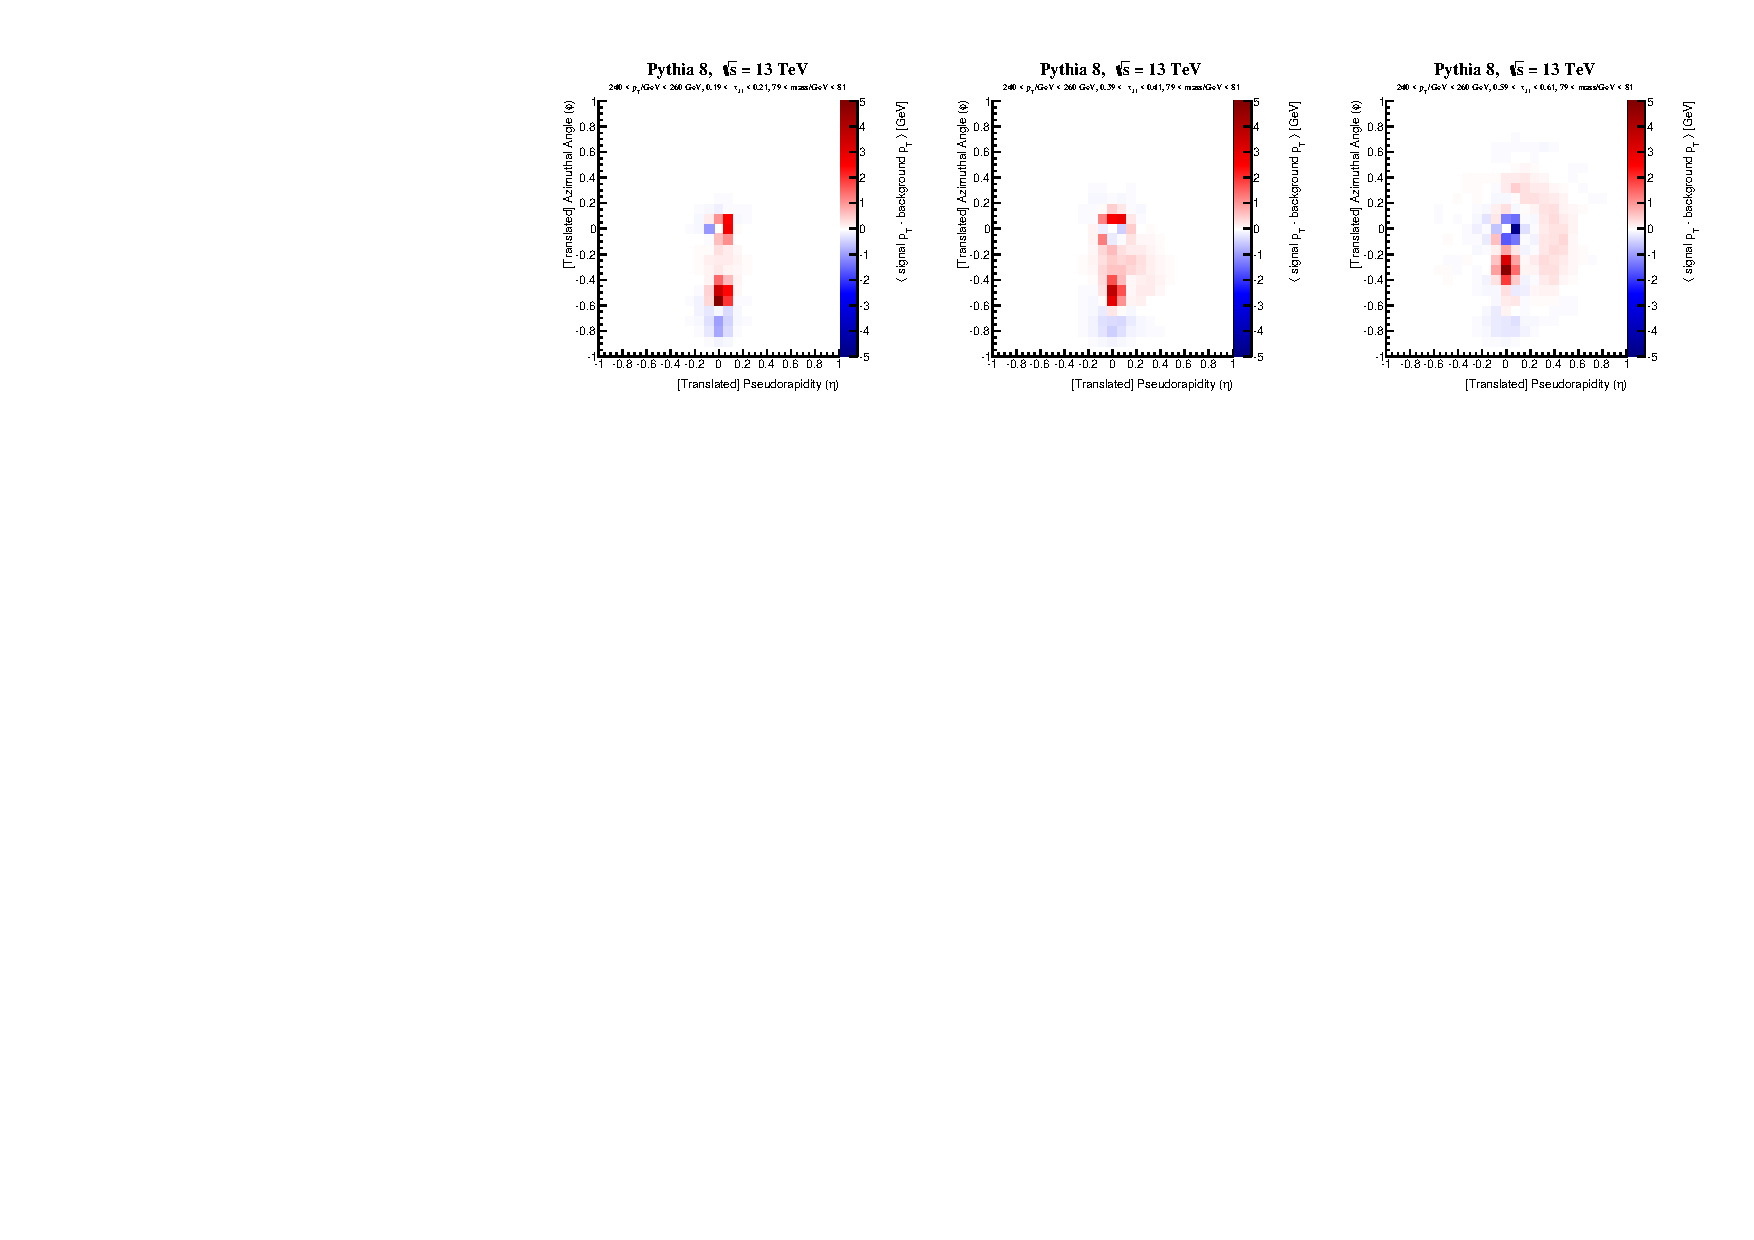
\includegraphics[width=0.99\textwidth]{figures/difference_fixed_nonorm.pdf}
        
      \caption{
         The average difference between $W'\rightarrow WZ$ jet-images in three small windows of $\tau_{21}$: [0.19, 0.21] (left), [0.39, 0.41] (middle), and [0.59, 0.61] (right).  In all cases, jet mass is restricted to be between 79 GeV and 81 GeV and the jet $p_T$ is required to be in the interval [250,260] GeV.  The red colors are more signal-like and the blue is more background-like.
        \label{fig:meanImagesWindow2} 
      }
    \end{center}
\end{figure}  

\begin{figure}[htbp]
  \centering
  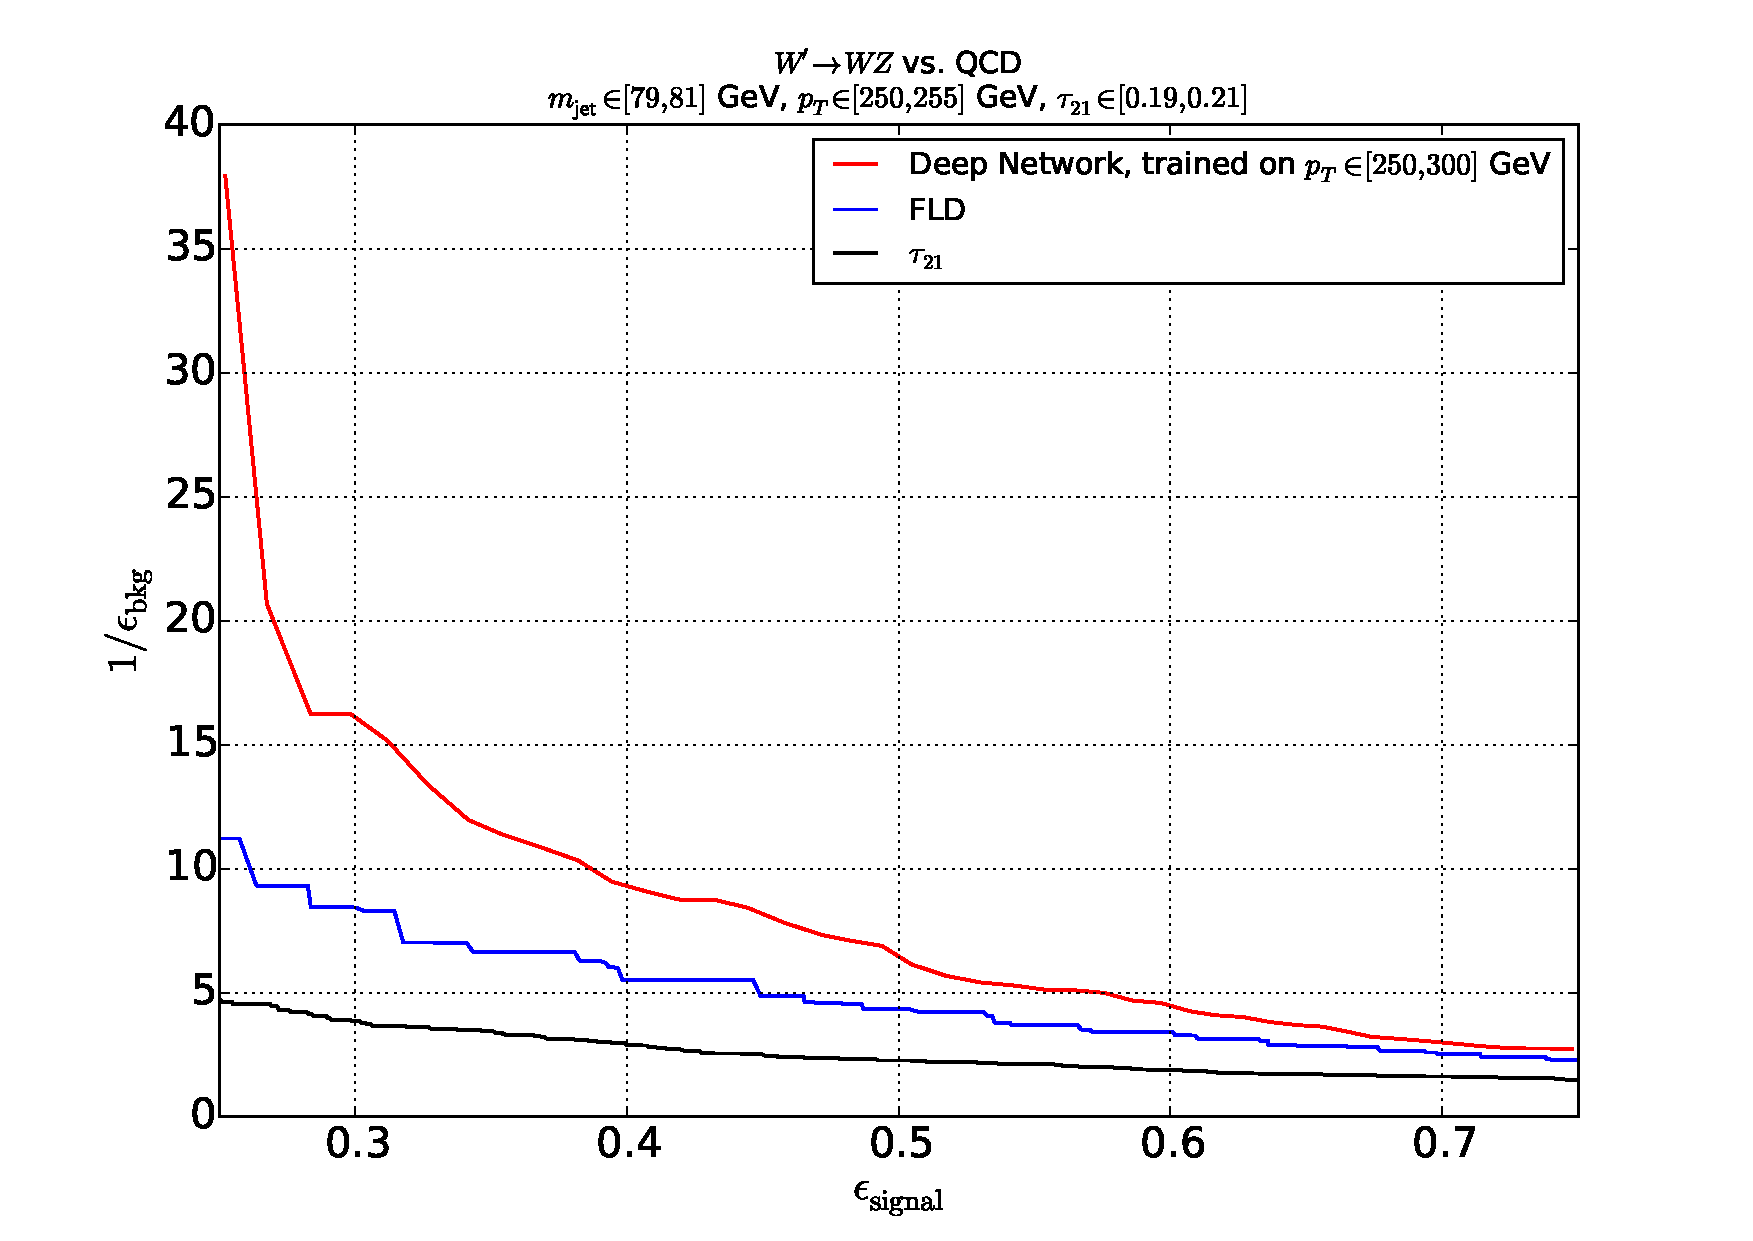
\includegraphics[width=0.5\textwidth]{figures/augwindow-roc.pdf}
  \caption{Receiver Operating Characteristic (ROC) over window sample}
  \label{fig:rocWindow}
\end{figure}

%\subsubsection{Understanding what we learn} % (fold)
%\label{ssub:understanding_what_we_learn}

Now, we turn back to the neutral network and their performance in these small windows of jet mass and $\tau_{21}$.    Figure~\ref{fig:rocWindow} shows three ROC curves in the window $\tau_{21} \in[0.19,0.21].  By construction, the $\tau_{21}$ curve is no better than a random guess, since this variable does not significantly vary over the small window.  The other two curves are a Fisher Linear Discriminant\footnote{There is no $\Delta R$ binning as in the Fisher Jets of X, but this will make no difference since the $\Delta R$ distribution does not signficantly compared with the courase $\Delta R$ bins within the small mass and $p_T$ windows.} (FLD)

In this window, we compare the DNN trained outside the window to a Fisher Linear Discriminant trained inside the window. In Figure~\ref{fig:rocWindow} we see this performance comparison, and note that our DNN outperforms the FLD.

\begin{figure}[htbp]
  \centering
  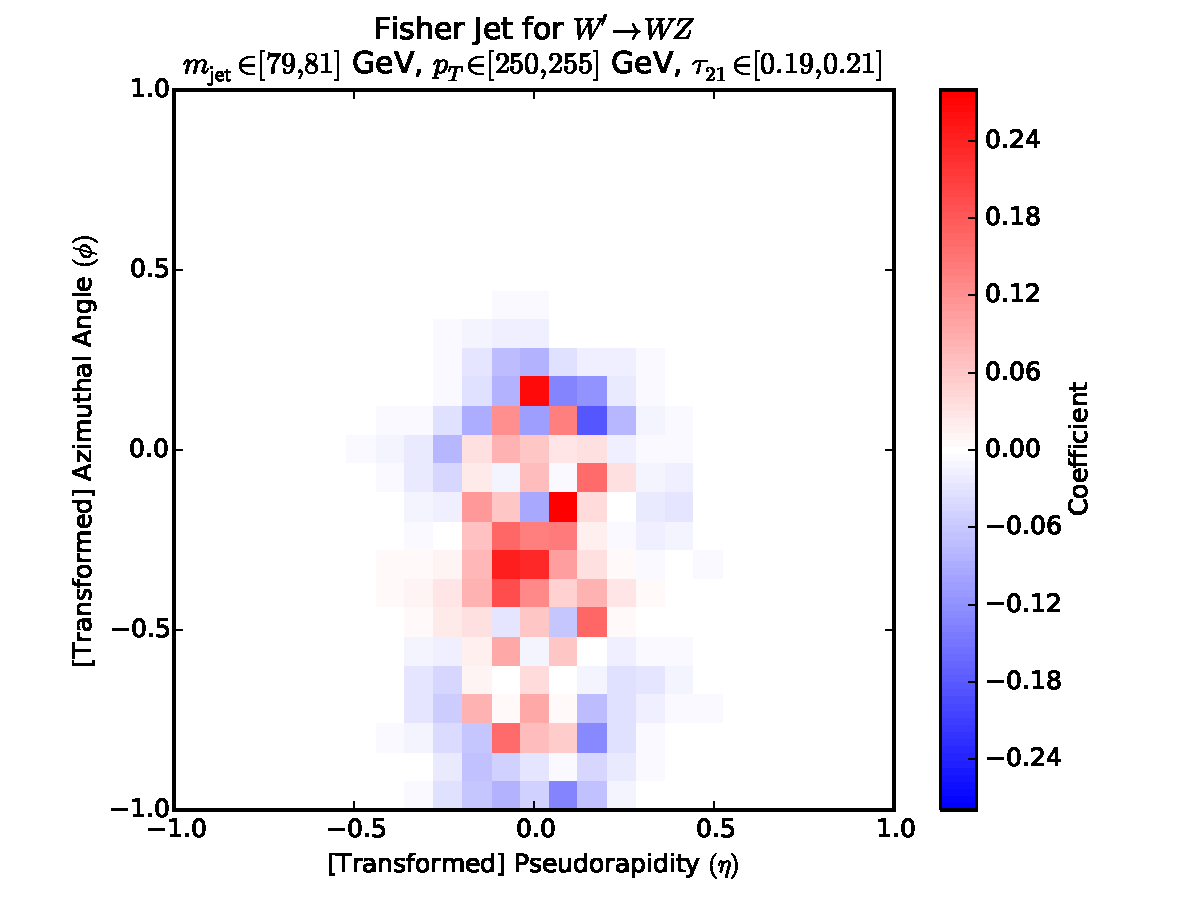
\includegraphics[width=0.65\textwidth]{figures/fld-benwindow.pdf}
  \caption{Cell coefficients from Fisher Linear Discriminant in window: $m_\text{jet}\in [79, 81]$ GeV, $p_{T}\in [250, 255]$ GeV, $\tau_{21}\in[0.19, 0.21]$}
  \label{fig:fldWindow}
\end{figure}

\begin{figure}[htbp]
  \centering
  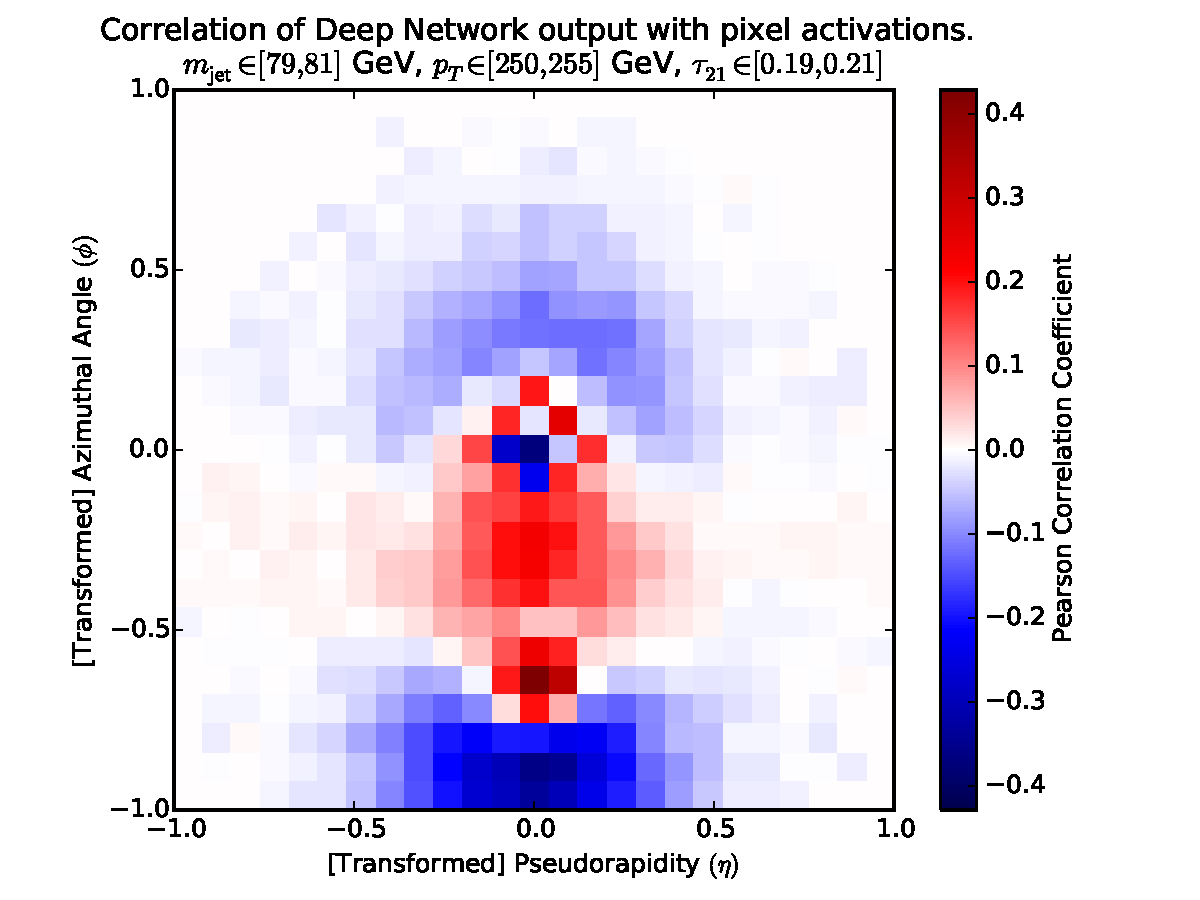
\includegraphics[width=0.65\textwidth]{figures/pixel-activations-corr-benwindow.pdf}
  \caption{Pearson Correlation Coefficient for pixels vs. DNN output, $m_{\mathsf{jet}}\in [79, 81]$ GeV, $p_{T}\in [250, 255]$ GeV, $\tau_{21}\in[0.19, 0.21]$}
  \label{fig:corrWindow}
\end{figure}

%In Figure~\ref{fig:convkernelsWindow}, we show the same feature representations as in Figure~\ref{subfig:convolvedfilters}, which show the convolved differences in images over signal and background in the window. 
%
%\begin{figure}[htbp]
%  \centering
%  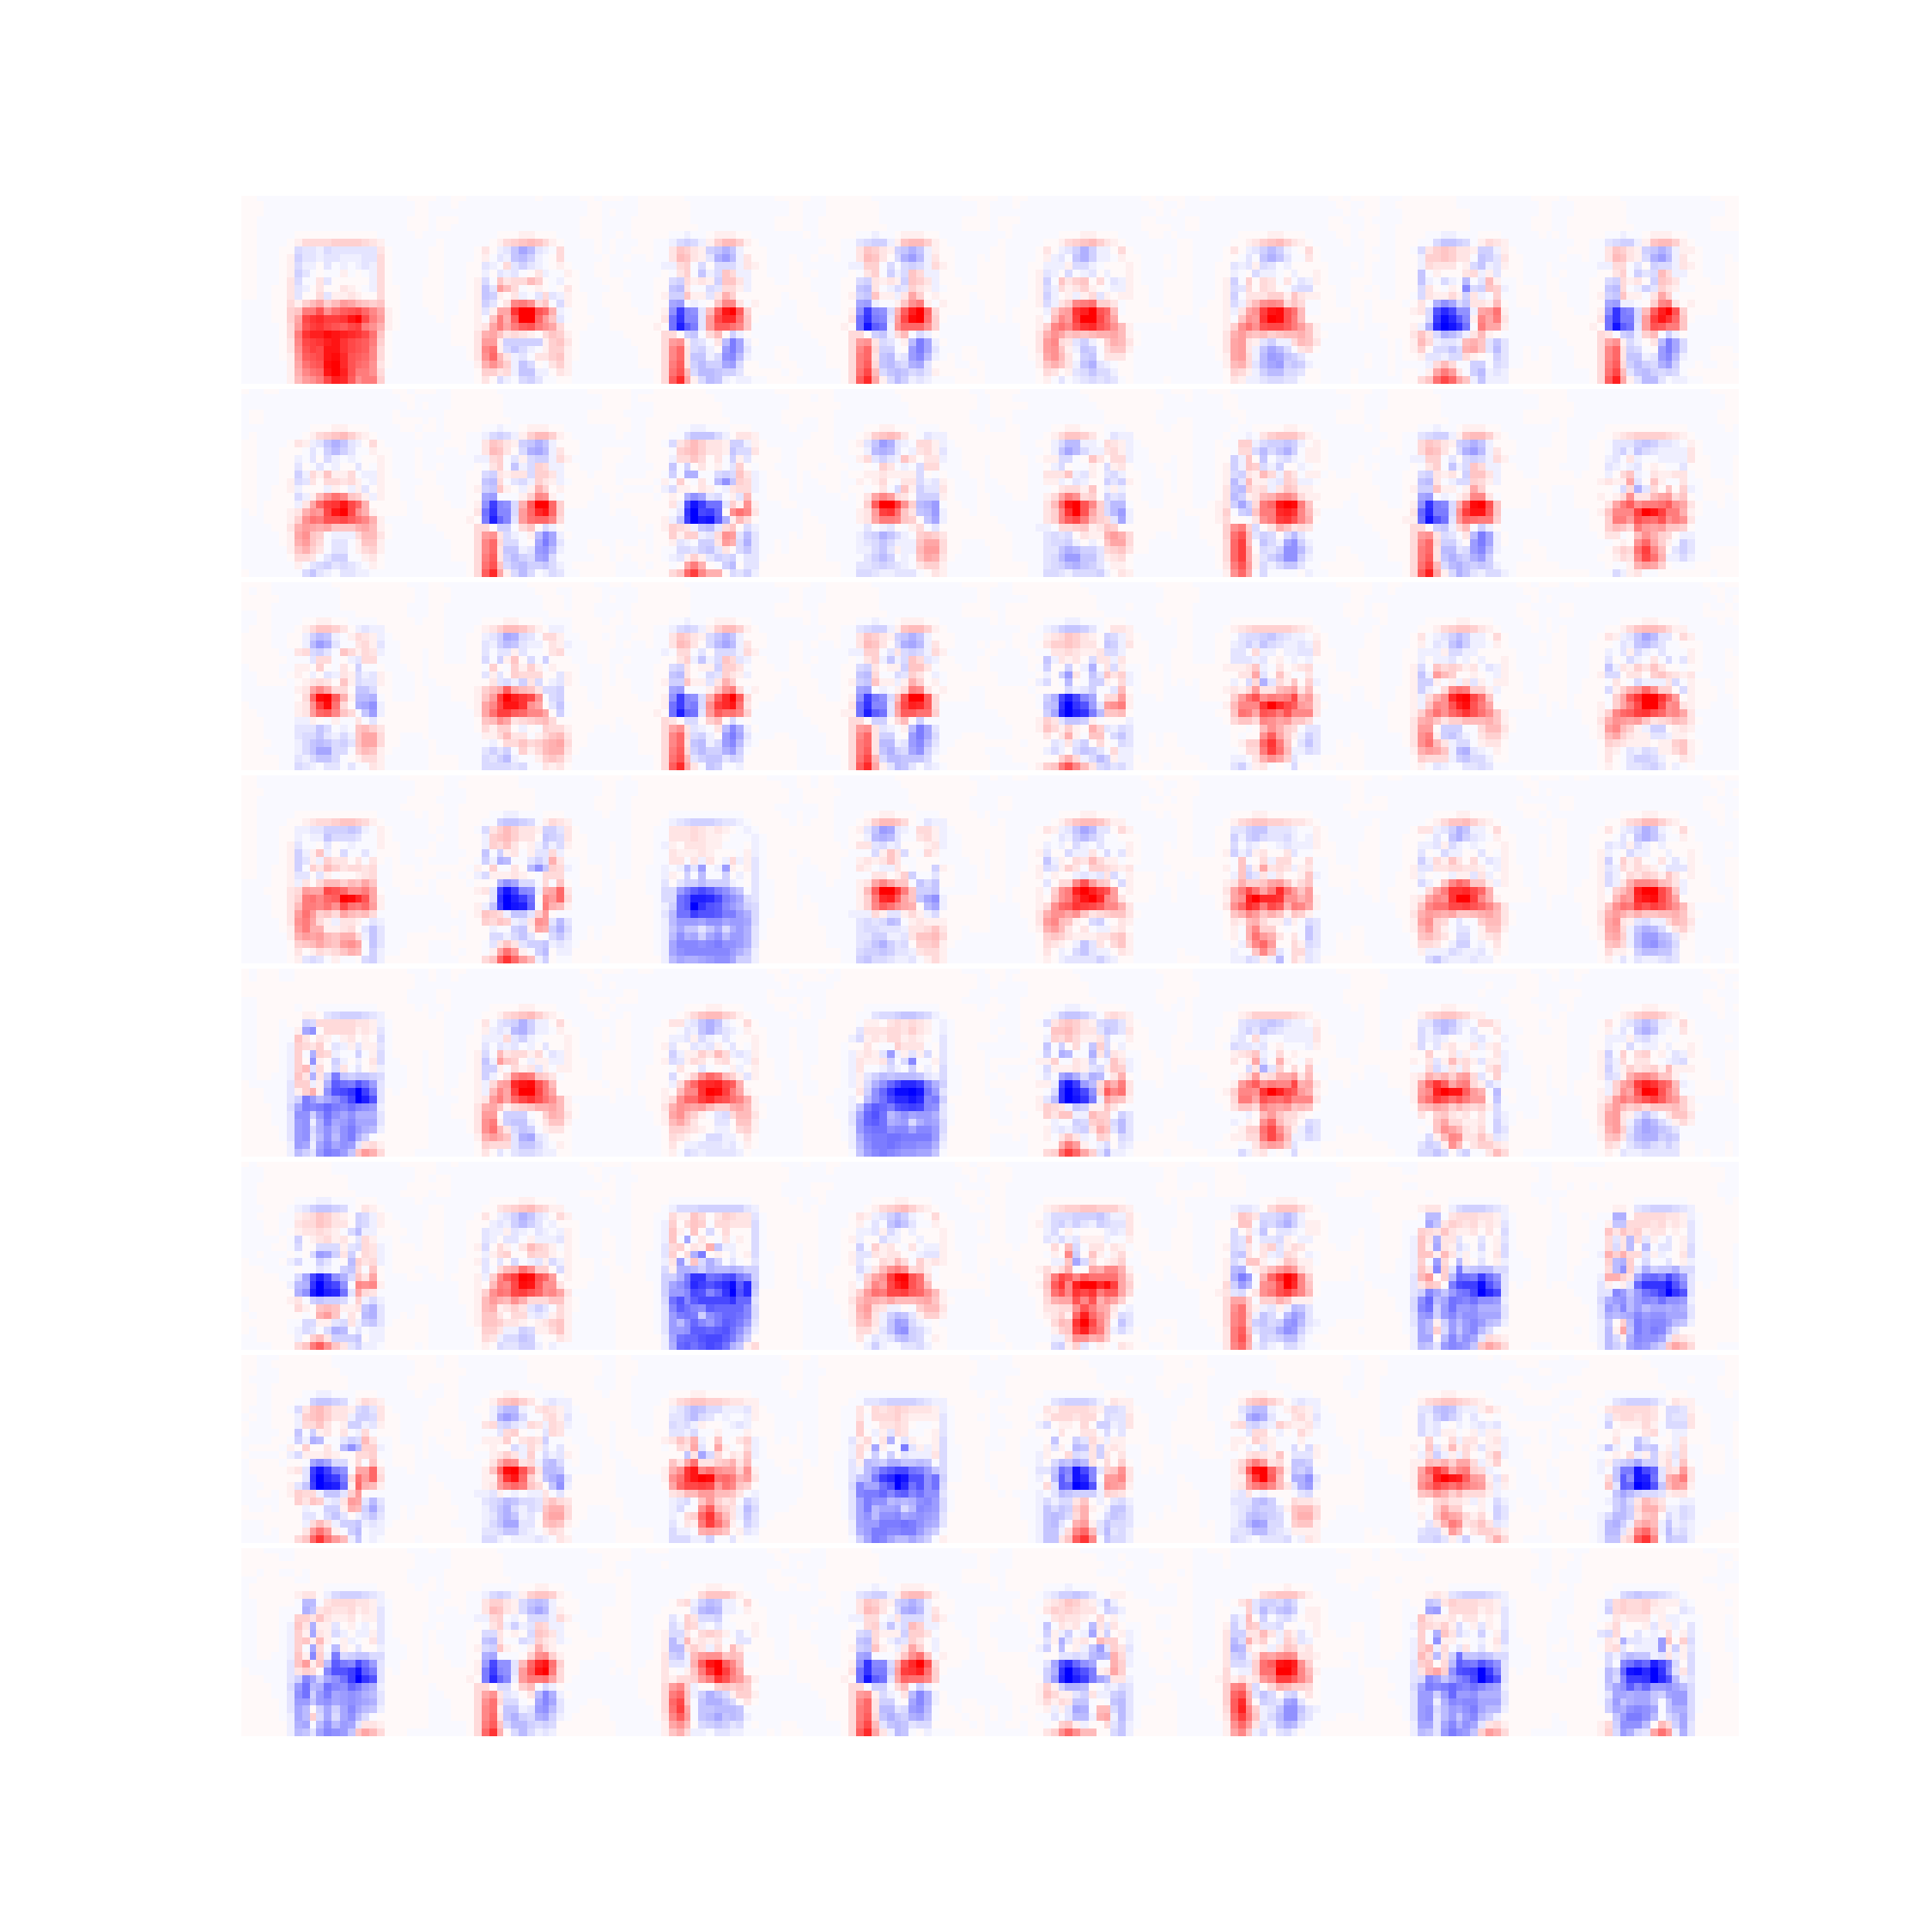
\includegraphics[width=0.95\textwidth]{figures/conv-diffs-ben-window.pdf}
%  \caption{Convolved Feature Differences in jet images, $m_\text{jet}\in [79, 81]$ GeV, $p_{T}\in [250, 255]$ GeV, $\tau_{21}\in[0.19, 0.21]$}
%  \label{fig:convkernelsWindow}
%\end{figure}


% subsubsection understanding_what_we_learn (end)

% subsection small_window_studies (end)

